% ApexS IEEE paper source — ENHANCED VERSION
% Compile with a standard IEEEtran-enabled LaTeX installation:
%   pdflatex APEX_S_IEEE_Paper.tex
%   bibtex   APEX_S_IEEE_Paper
%   pdflatex APEX_S_IEEE_Paper.tex
%   pdflatex APEX_S_IEEE_Paper.tex
%
% Replace the boxed placeholders with actual screenshots/figures before final submission.

\documentclass[conference]{IEEEtran}

\usepackage{cite}
\usepackage{amsmath,amssymb,amsfonts}
\usepackage{graphicx}
\usepackage{booktabs}
\usepackage{tabularx}
\usepackage{array}
\usepackage{multirow}
\usepackage{pgfplots}
\usepackage{pgfplotstable}
\usepackage{tikz}
\usepackage{enumitem}
\usepackage{xcolor}
\usepackage{balance}
\usepackage{algorithm}
\usepackage{algpseudocode}
\usepackage{soul}
\usepackage{microtype}
\usepackage{hyperref}

\pgfplotsset{compat=1.18}
\usetikzlibrary{shapes.geometric, arrows.meta, positioning, fit, backgrounds, calc}

\hypersetup{
  colorlinks=true,
  linkcolor=black,
  citecolor=black,
  urlcolor=blue
}

\newcolumntype{Y}{>{\raggedright\arraybackslash}X}
\newcolumntype{C}{>{\centering\arraybackslash}X}

% ── Placeholder helpers ────────────────────────────────────────────────────────
\newcommand{\placeholderfig}[2]{%
  \fbox{%
    \parbox[c][1.45in][c]{0.94\columnwidth}{%
      \centering
      \textbf{Image Placeholder}\\[4pt]
      #1\\[6pt]
      \footnotesize #2
    }%
  }%
}

\newcommand{\placeholderwidefig}[2]{%
  \fbox{%
    \parbox[c][1.8in][c]{0.97\textwidth}{%
      \centering
      \textbf{Wide Image Placeholder}\\[4pt]
      #1\\[6pt]
      \footnotesize #2
    }%
  }%
}

% ── Title ─────────────────────────────────────────────────────────────────────
\title{ApexS: Explainable Context-Aware Sprint Planning with Learned Team Weights,
       Constraint-Aware MILP Optimization, and End-to-End Decision Support}

\author{
\IEEEauthorblockN{Midhul Kiruthik M\textsuperscript{\dag},
                  Madhan Karthikeyan,
                  Manav Kaizen,
                  Sharvesh S}
\IEEEauthorblockA{
School of Computer Science and Engineering,
Vellore Institute of Technology, Chennai, India \\
Team ApexS, BCSE301P Software Engineering Lab, Winter Semester 2025--26 \\
Reg.\ Nos.: 23BCE0783\textsuperscript{\dag}, 23BCE0829, 23BCE2251, 23BCE2141 \\
\textsuperscript{\dag}Team Leader
}
}

\begin{document}

\maketitle

% ══════════════════════════════════════════════════════════════════════════════
\begin{abstract}
Sprint planning remains difficult because value, effort, risk, skill availability,
and dependency structure must be reconciled under time pressure, yet many planning
tools still rely on manual prioritization or opaque heuristics.
%
This paper presents \textbf{ApexS}, an explainable context-aware sprint planning
system implemented as a full-stack decision-support platform with a FastAPI backend,
React frontend, asynchronous planning orchestration with Celery integration,
dataset conversion and cleaning scripts, and a mixed-integer linear programming
(MILP) optimization core built on PuLP/CBC.
%
The implemented pipeline learns team-specific \emph{urgency}, \emph{value}, and
\emph{alignment} weights from historical sprint data via Ridge regression, enforces
four hard planning constraints (capacity, risk threshold, skill compatibility, and
dependency satisfaction) through status-aware feasibility filtering and
dependency-aware binary optimization, and generates story-level explanations for
both selected and rejected items.
%
The system follows a five-layer modular architecture (Presentation, Application,
Data, Worker, and Storage) deployed as a reproducible six-service Docker Compose
stack, and exposes a versioned REST API covering the complete planning lifecycle
from dataset upload to Jira-compatible export.
%
The empirical evaluation is organized around four cleaned Jira-derived datasets:
Spring XD, Usergrid, Aurora, and TAWOS, with TAWOS serving as the primary
real-world validation corpus.
Across these four frozen CSV snapshots, the current paper-ready dataset pool
contains 19,095 stories and 487 sprint groups in total; TAWOS alone contributes
14,738 stories and 673 dependency-bearing rows.
The manuscript is structured so that dataset-level characteristics, planning
performance, baseline comparison, distributional analysis, and qualitative
case-study evidence can all be reported consistently across the same four corpora.
%
All 20 automated tests passed in the recorded verification snapshot, and the
repository includes a working dataset converter, multiple pre-validated
upload-ready datasets, and a complete approval-and-export workflow.
%
The main novelty lies in integrating learned weighting, constraint-aware MILP
selection, bidirectional explanation generation, and approval/export support into
one reproducible engineering pipeline that extends the ASE 2024 context-aware
sprint planning baseline with explicit risk-awareness, skill-awareness, and
decision traceability.
\end{abstract}

\begin{IEEEkeywords}
agile sprint planning, mixed-integer linear programming, explainable AI for
software engineering, Jira datasets, decision support systems, software engineering
analytics, Ridge regression, backlog optimization, constraint satisfaction
\end{IEEEkeywords}

% ══════════════════════════════════════════════════════════════════════════════
\section{Introduction}
\label{sec:intro}

Sprint planning directly determines what a software team attempts during the next
iteration, yet the underlying decision process is rarely treated as a rigorous
optimization-and-explanation problem.
Teams must balance business value, schedule pressure, implementation effort,
technical risk, required skills, and dependency feasibility while also preserving
enough transparency for product owners and Scrum masters to trust the result.
In practice, these decisions are often made through manual triage, spreadsheet
scoring, or simple ranking rules, all of which struggle when the backlog grows or
when historical sprint data exists but is not operationalized.

Recent work has shown that optimization can support agile planning, and that richer
project datasets can improve decision quality and empirical evaluation
\cite{ase2024, agile-mo, tawos, jira-dataset}.
At the same time, explainable AI has become increasingly important in software
engineering because stakeholders must understand why a model or recommender made a
specific decision \cite{xai-slr-se, xai-survey, explanation-matters}.
However, most prior studies stop short of an end-to-end implementation that couples
learned team behavior, hard operational constraints, and per-story explanations
inside one deployable planning loop.

This paper addresses that gap through \textbf{ApexS}, a repository-backed system
built around four design goals.
First, planning should be \emph{context-aware}: historical sprint data should
influence the relative importance of urgency, value, and alignment.
Second, planning should be \emph{constraint-consistent}: infeasible stories should
be removed or constrained before selection.
Third, planning should be \emph{explainable}: both acceptance and rejection should
be auditable at story level with human-readable justifications and confidence
scores.
Fourth, planning should be \emph{operational}: the system should support upload,
optimization, explanation review, approval, and export without leaving the
application.

ApexS directly extends the ASE 2024 context-aware sprint planning baseline
\cite{ase2024} by adding four contributions that were absent from the base work:
team-specific weight learning from historical outcomes, four simultaneous hard
constraints in one ILP formulation, per-story bidirectional explainability, and a
complete approval-and-export decision support loop.

To sharpen the empirical focus, the paper studies three research questions.
\textbf{RQ1}~(Feasibility): can a learned-weight MILP formulation produce plans
that remain operationally feasible under realistic capacity, risk, skill, and
dependency constraints?
\textbf{RQ2}~(Explainability): does the implemented explanation layer provide
complete and decision-specific coverage for both accepted and rejected stories?
\textbf{RQ3}~(Comparative): does the integrated system outperform a simpler
value-first feasible ranking baseline on representative sprint-ready backlogs?
These questions align with the codebase itself: the repository implements learning,
optimization, explanation, and workflow support as distinct yet connected stages, so
the paper evaluates the system at the same granularity.

The contributions of this work are:
\begin{enumerate}[leftmargin=*,itemsep=1pt,topsep=2pt]
\item A full-stack sprint planning system that integrates dataset ingestion, context
      extraction, weight learning, MILP optimization, explanation generation, and
      approval/export workflow in one reproducible Docker Compose stack.
\item A repository-grounded planning formulation that matches the implemented code
      path, including status-aware feasibility filtering, risk gating, skill
      compatibility filtering, and dependency constraints.
\item A quantitative evaluation combining historical-data diagnostics,
      scenario-based planning metrics, latency measurements, and recorded system
      verification evidence.
\item A clear novelty layer over prior sprint-planning studies: learned
      team-specific weights, bidirectional explanation output (selected and
      rejected), and an end-to-end decision-support loop rather than an isolated
      optimizer.
\item A validated dataset processing pipeline with converter scripts, multiple
      pre-validated upload-ready datasets, and a schema that matches the Jira
      export format used in industry.
\end{enumerate}

The remainder of this paper is structured as follows.
Section~\ref{sec:related} surveys related work.
Section~\ref{sec:requirements} describes the system requirements and process model.
Section~\ref{sec:methodology} presents the architecture and methodology.
Section~\ref{sec:results} reports evaluation results and discussion.
Section~\ref{sec:conclusion} concludes with future directions.

% ══════════════════════════════════════════════════════════════════════════════
\section{Literature Survey}
\label{sec:related}

Optimization support for sprint planning has matured from heuristic formulations
toward more context-sensitive backlog selection.
Ozcelikkan~\emph{et al.} proposed a multi-objective agile project planning model
and demonstrated that mathematically grounded planning can outperform naive
prioritization under competing objectives \cite{agile-mo}.
Kula~\emph{et al.} later extended the discussion by introducing context-aware
sprint plan generation, showing that planning quality improves when project context
is modeled rather than assumed static \cite{ase2024}.
These studies motivate the use of formal optimization but do not fully resolve the
engineering problem of exposing decisions, collecting evidence, and integrating the
workflow with a usable planning system.

Chaves~\emph{et al.}\ proposed a Lagrangian heuristic for sprint planning that
explicitly formulates backlog selection as a constrained combinatorial problem
\cite{lagrangian-sprint}.
Their work confirms the feasibility of mathematical programming for agile planning
but addresses neither explainability nor team-adaptive weighting.

Public datasets have also improved empirical rigor.
TAWOS offers a structured dataset of agile open-source projects \cite{tawos},
while the public Jira repository dataset released by Montgomery~\emph{et al.}
provides issue-level information that is especially useful for backlog, workflow,
and dependency analysis \cite{jira-dataset}.
Complementary studies on intelligent software engineering in agile contexts and on
agile data analytics show that historical project traces can support prioritization,
estimation, and reporting, but they also highlight the fragmentation between
isolated analytics and deployable tools \cite{intelligent-agile, bigdata-agile}.

Effort estimation studies are relevant because sprint planning relies on credible
effort signals.
Transformer-based story point estimation \cite{gpt2sp}, ensemble-based story point
prediction \cite{ensemble-spe}, and large language model studies on agile effort
estimation \cite{llm-effort} collectively indicate that machine learning can
capture regularities in agile artifacts.
Yet these methods typically optimize estimation accuracy rather than final
sprint-feasibility decisions.
Similarly, systematic mappings of early estimation in agile projects show that
estimation support is abundant, but integrated planning pipelines remain limited
\cite{agile-estimation-map}.

Risk modeling in software projects is a further relevant strand.
Bug triage datasets and defect prediction studies \cite{bugtriage-deeplearning}
demonstrate that historical defect history can provide proxy signals for story-level
risk, which ApexS exploits through its dataset converter pipeline.
Integrating such signals into a planning optimizer---rather than treating them as
independent prediction tasks---is one of the open engineering challenges that ApexS
begins to address.

Explainability is increasingly necessary in software engineering tools.
General XAI surveys document the trade-off between model performance and
interpretability \cite{xai-survey}, while explanation studies show that user trust
depends on explanation quality and task context \cite{explanation-matters}.
In software engineering specifically, Mohammadkhani~\emph{et al.} identify a
shortage of explainable systems that move beyond conceptual proposals and operate
on real engineering data \cite{xai-slr-se}.
ApexS is positioned within this gap: it combines learned weighting, hard constraint
enforcement, and user-facing explanations in a system that can actually be run,
tested, and audited.

Table~\ref{tab:related-comparison} positions ApexS against representative prior
systems along the four dimensions that define its design goals.

\begin{table}[t]
\caption{Positioning ApexS Against Representative Prior Work}
\label{tab:related-comparison}
\centering\small
\begin{tabularx}{\columnwidth}{lYYYY}
\toprule
System & Team-adapt & 4 constraints & Bidirectional explain & Full workflow \\
\midrule
ASE 2024 \cite{ase2024}       & Partial & No  & No  & No  \\
Lagrangian \cite{lagrangian-sprint} & No & Partial & No & No  \\
MO-agile \cite{agile-mo}       & No     & No  & No  & No  \\
GPT2SP \cite{gpt2sp}           & No     & No  & No  & No  \\
\textbf{ApexS (this work)}     & \textbf{Yes} & \textbf{Yes} & \textbf{Yes} & \textbf{Yes} \\
\bottomrule
\end{tabularx}
\end{table}

Across these strands, the unresolved gap is not merely algorithmic accuracy.
The more difficult research problem is how to transform noisy project history into a
plan that is simultaneously feasible, inspectable, and usable inside a real sprint
workflow.
That is the level at which ApexS contributes: it operationalizes the analytics
pipeline rather than presenting isolated prediction or optimization components.

% ══════════════════════════════════════════════════════════════════════════════
\section{System Requirements and Process Model}
\label{sec:requirements}

\subsection{Functional Requirements}

The system was specified using the IEEE~830 SRS format prior to implementation.
Eight functional requirements (F1--F8) drive the design:

\begin{enumerate}[leftmargin=*,itemsep=1pt,topsep=2pt,label={F\arabic*.}]
\item \emph{Dataset Import}: upload historical sprint data in CSV format with
      schema validation (required columns: \texttt{story\_id},
      \texttt{story\_points}, \texttt{business\_value}, \texttt{risk\_score}).
\item \emph{Context Extraction}: compute velocity, completion rate, skill
      distribution, and feature correlations from uploaded history.
\item \emph{Weight Learning}: infer team-specific urgency, value, and alignment
      weights from historical completion outcomes.
\item \emph{MILP Optimization}: generate optimized sprint backlogs subject to
      configurable constraints with MILP optimization and a greedy fallback path
      when the MILP solver is unavailable or does not return an optimal solve.
\item \emph{Risk Awareness}: enforce a configurable risk-score threshold as a hard
      feasibility constraint before optimization and preserve that filtered set in
      the optimization stage.
\item \emph{Explainability}: generate per-story acceptance/rejection reasons,
      contribution breakdowns, and confidence scores.
\item \emph{Modification}: re-run optimization from an existing plan with updated
      constraint parameters to support what-if analysis.
\item \emph{Reporting}: surface velocity trends, value delivery trends, risk
      profiles, and learning-model diagnostics.
\end{enumerate}

Table~\ref{tab:req-traceability} shows how each requirement maps to the implemented
system component.

\begin{table}[t]
\caption{Requirements-to-Implementation Traceability Matrix}
\label{tab:req-traceability}
\centering\small
\begin{tabularx}{\columnwidth}{lY}
\toprule
Requirement & Implementing Component \\
\midrule
F1 Import Data      & \texttt{ContextExtractor} + Dataset Upload API \\
F2 Context Analysis & \texttt{ContextExtractor} \\
F3 Learn Weights    & \texttt{WeightLearningModel} (Ridge regression) \\
F4 Optimization     & \texttt{OptimizationEngine} (PuLP/CBC) \\
F5 Risk Awareness   & Feasibility filter + C2 constraint in MILP \\
F6 Explainability   & \texttt{ExplainabilityEngine} \\
F7 Modification     & Plans API + \texttt{OptimizationEngine} re-run \\
F8 Reporting        & Reports API + Report Viewer UI \\
\bottomrule
\end{tabularx}
\end{table}

\subsection{Non-Functional Requirements}

Key non-functional constraints include: plan generation within 60~s for backlogs
up to 100 stories (Performance); best-effort fallback plan on infeasibility rather
than server error (Reliability); human-readable explanations accessible from both
API and UI (Usability); single-command full-stack deployment via Docker Compose
(Portability); and JWT-based role-level authentication for Scrum Master and Product
Owner roles (Security).

\subsection{Process Model}

ApexS adopts the \emph{Agile Scrum} process model as its development methodology,
for reasons that are intrinsic to the problem domain.
The system is designed to operate \emph{within} the Scrum framework---specifically
targeting the Sprint Planning ceremony---so development itself followed the same
incremental sprint structure.
Each development sprint mapped to one implementation phase: Sprint 0 (infrastructure
and scaffolding), Sprint 1 (data ingestion and context extraction), Sprint 2 (MILP
engine), Sprint 3 (explainability), Sprint 4 (frontend integration), and Sprint 5
(evaluation and documentation).

This alignment between development process and research subject is intentional.
It allowed the team to validate design decisions at each increment rather than
accumulating risk toward a single integration point.
Heavyweight sequential models such as Waterfall were rejected because research
requirements evolved as empirical results became available.
Microservices architecture was rejected for operational simplicity: the six-service
Docker Compose stack provides sufficient isolation without the overhead of
inter-service contract management.

% ══════════════════════════════════════════════════════════════════════════════
\section{Methodology}
\label{sec:methodology}

\subsection{System Architecture and Overview}

ApexS follows a five-layer modular architecture: (1)~\emph{Presentation Layer}
(React~18 + TypeScript frontend with Vite and React Query); (2)~\emph{Application
Layer} (FastAPI service with versioned REST API at \texttt{/api/v1}); (3)~\emph{Worker
Layer} (Celery task with Redis broker, executing the planning pipeline
asynchronously); (4)~\emph{Data Layer} (SQLAlchemy ORM over SQLite in development
or PostgreSQL in production, with Alembic migrations); and (5)~\emph{Storage Layer}
(MinIO for CSV/JSON file objects).

The full Docker Compose stack comprises six services: \texttt{frontend},
\texttt{backend}, \texttt{db} (PostgreSQL), \texttt{redis}, \texttt{minio}, and
\texttt{celery\_worker}.
After a single \texttt{docker compose up --build}, the system is accessible at
four endpoints: frontend UI at \texttt{:5173}, backend API at \texttt{:8000}, API
documentation (Swagger) at \texttt{:8000/docs}, and MinIO console at
\texttt{:9001}.

The backend exposes 18 versioned REST endpoints across seven route groups:
\texttt{/auth}, \texttt{/teams}, \texttt{/datasets}, \texttt{/sprints},
\texttt{/stories}, \texttt{/plans}, and \texttt{/reports}.
Plan generation is triggered asynchronously: \texttt{POST /plans/generate} returns
a \texttt{job\_id} immediately, and the caller polls
\texttt{GET /plans/status/\{job\_id\}} until \texttt{status = done}.
This prevents blocking the UI during ILP solve time and enables real-time progress
reporting.

\begin{figure*}[t]
\centering
\IfFileExists{figs/architecture.png}{%
  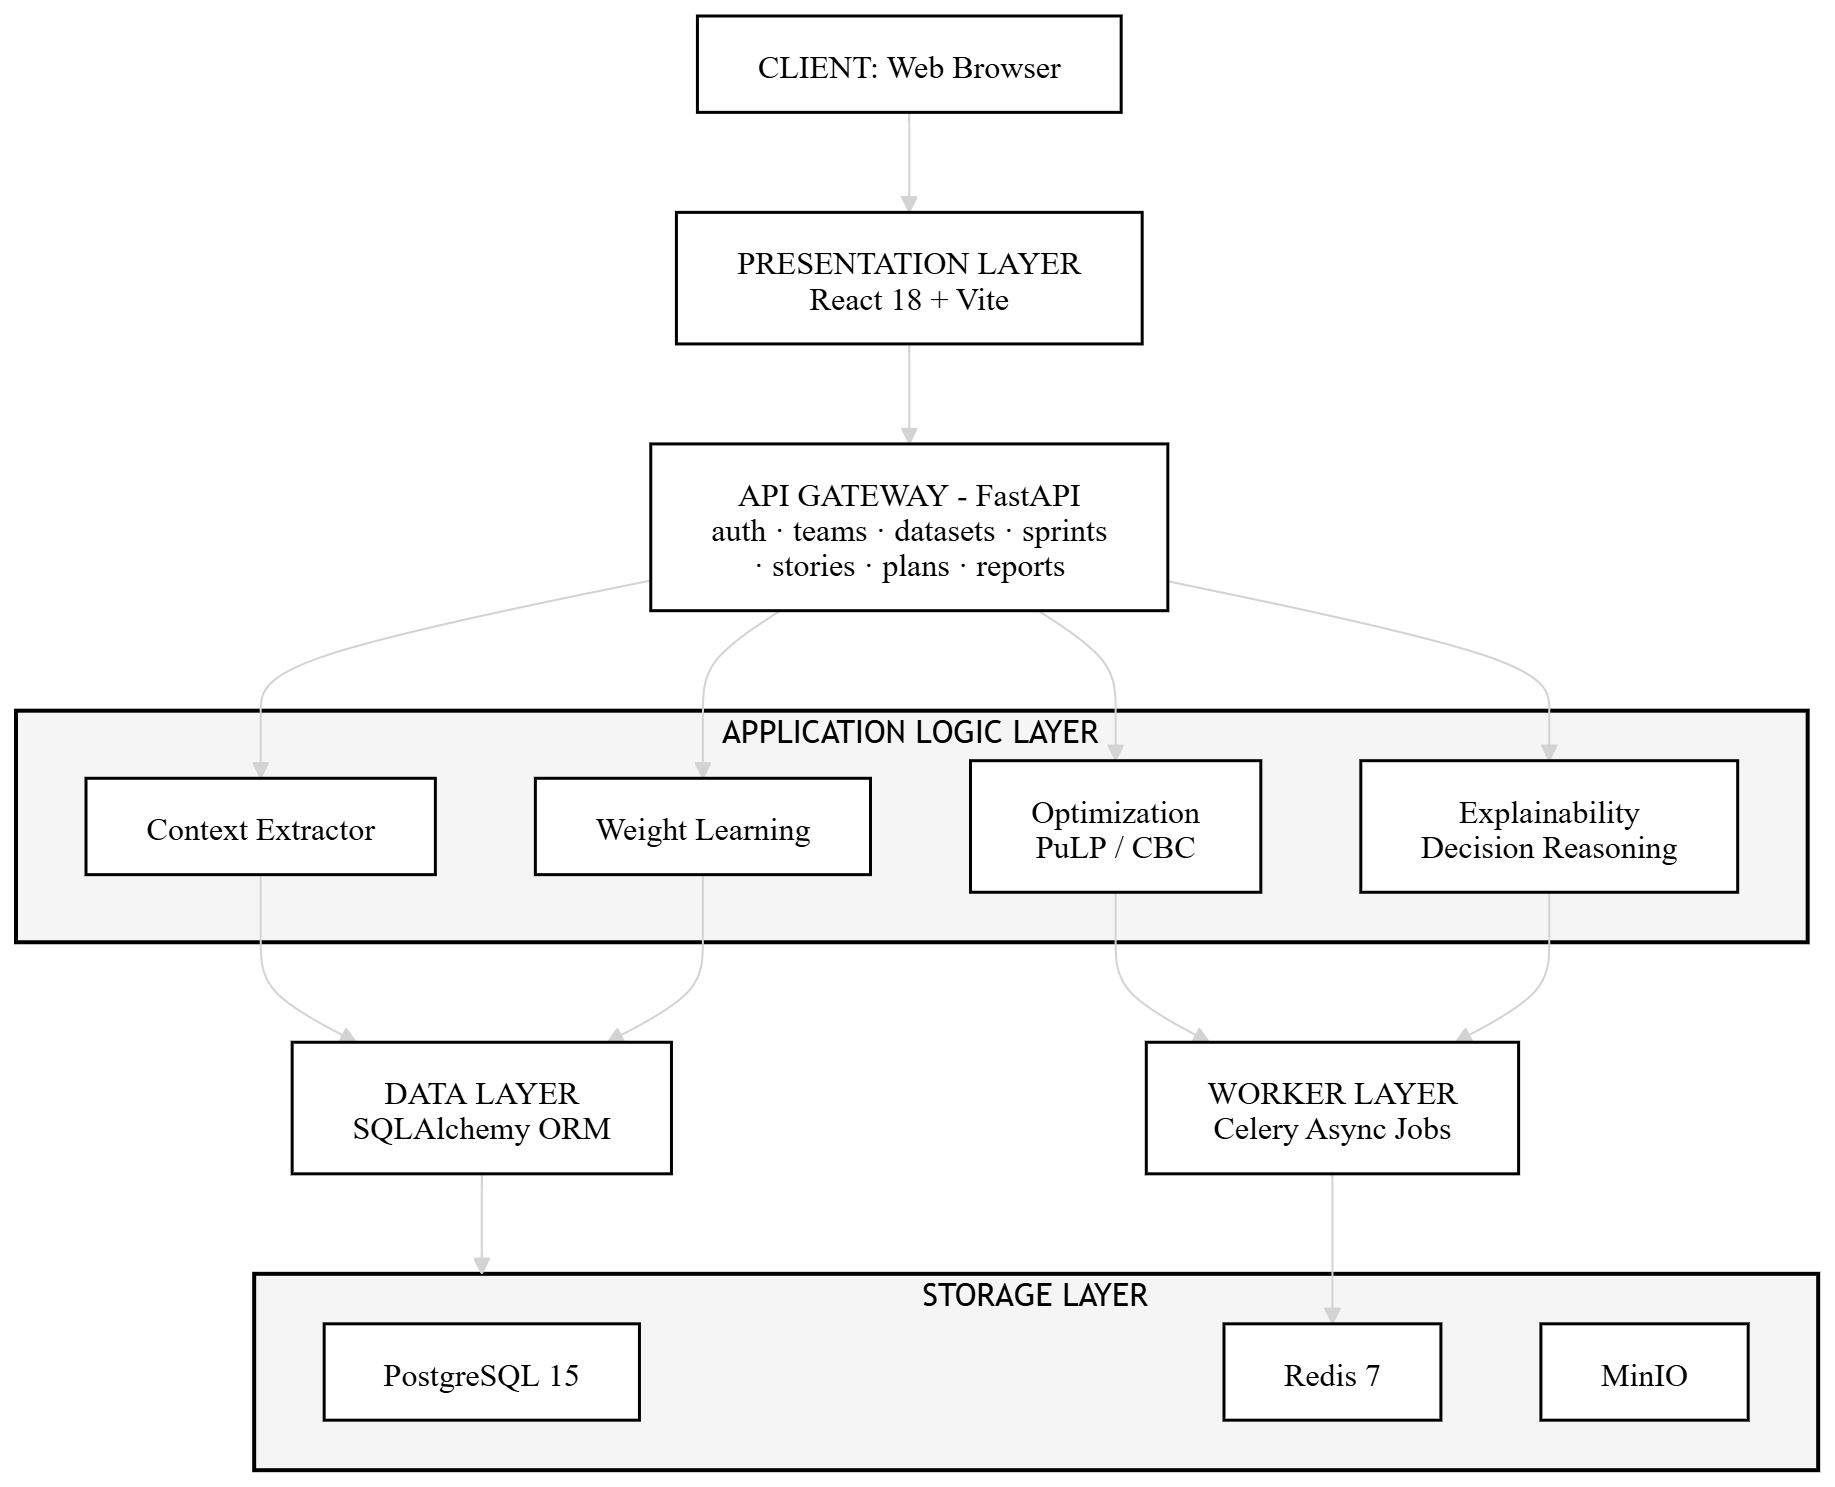
\includegraphics[width=0.97\textwidth]{figs/architecture.png}%
}{%
  \placeholderwidefig{Five-layer modular architecture of the ApexS sprint planning stack.}{Replace with actual architecture diagram before submission.}%
}
\caption{Five-layer modular architecture of the ApexS sprint planning stack.
         Layers from top to bottom: (1)~Presentation Layer with React~18 frontend,
         (2)~Application Layer exposing seven FastAPI route groups for team/dataset/plan
         management, including four core application services (Optimization via
         PuLP/CBC, Explainability engine, Context extractor, and Weight learner),
         (3)~Worker Layer using Celery with Redis broker for long-running planning tasks,
         (4)~Data Layer with SQLAlchemy ORM and Alembic-managed migrations, and
         (5)~Storage Layer using PostgreSQL, Redis, and MinIO.
         The planning pipeline (dataset upload $\rightarrow$ context extraction
         $\rightarrow$ weight learning $\rightarrow$ MILP optimization $\rightarrow$
         explanation generation) executes asynchronously in the Celery worker, with
         progress exposed through the Plans API.}
\label{fig:architecture}
\end{figure*}

The backend services that matter for the paper are directly implemented in the
repository.
\texttt{ContextExtractor} computes contextual weights and team statistics from
historical data.
\texttt{WeightLearningModel} fits a Ridge regression model over story points,
business value, and risk score to infer urgency, value, and alignment weights.
\texttt{OptimizationEngine} performs binary selection with PuLP/CBC.
\texttt{ExplainabilityEngine} produces human-readable reasons plus contribution
fields and confidence scores.
The planning worker orchestrates these stages and reports progress through named
steps: \texttt{loading}, \texttt{syncing\_stories}, \texttt{loading\_history},
\texttt{extracting}, \texttt{learning}, \texttt{optimizing}, \texttt{explaining},
and \texttt{done}.

\subsection{Dataset Processing Pipeline}

The repository includes dataset conversion and cleaning scripts so that
heterogeneous Jira-style exports can be transformed into the schema expected by the
planner.
The converter script maps common source fields such as \texttt{issue key},
\texttt{summary}, \texttt{priority}, and \texttt{story points} to a normalized CSV
with eleven columns: \texttt{story\_id}, \texttt{title}, \texttt{description},
\texttt{story\_points}, \texttt{business\_value}, \texttt{risk\_score},
\texttt{required\_skill}, \texttt{sprint\_id}, \texttt{sprint\_completed},
\texttt{depends\_on}, and \texttt{status}.
The cleaning script then standardizes statuses, derives or bounds risk and value,
infers required skills from textual cues, and removes duplicates.

For the final paper, the empirical study is restricted to four cleaned
Jira-derived datasets only:
\texttt{files/cleaned\_datasets/spring\_xd\_clean.csv},
\texttt{files/cleaned\_datasets/usergrid\_clean.csv},
\texttt{files/cleaned\_datasets/aurora\_clean.csv}, and
\texttt{tawos/paper\_datasets/tawos\_apex\_clean.csv}.
Spring XD, Usergrid, and Aurora are used as supporting comparative datasets,
whereas TAWOS is used as the primary real-world evaluation dataset because it
offers the largest corpus and the richest combination of sprint and dependency
evidence.

The same normalized schema is used across all four files, which allows a single
planning pipeline and a single reporting protocol to be reused throughout the
evaluation.
All descriptive statistics, optimization outcomes, baseline comparisons, and case
study examples reported in the paper should therefore be generated only from these
four frozen CSV snapshots.
Detailed corpus-level statistics are deferred to the Results section, where the
cross-dataset summary is reported in Table~\ref{tab:dataset-summary}.

\subsection{Context Extraction and Weight Learning}

The context extractor computes sprint-level statistics that serve two purposes:
they provide descriptive analytics for reporting and they initialize the
weight-learning stage with project-specific priors.
The implemented extractor computes mean velocity over sprint IDs, completion rate,
skill distribution, average tolerated risk among completed stories, and the
correlation between business value and completion.
Let $V$ denote mean sprint velocity, $\rho$ the value-completion correlation, $\bar{r}$
the mean risk of completed stories, and $C$ the target sprint capacity.
The extractor normalizes three contextual components:
\begin{equation}
\begin{aligned}
u &= \min(1,\; V/C), \\
v &= \min(1,\; \max(0.1,\; \rho + 0.5)), \\
a &= \min(1,\; \max(0.1,\; 1 - \bar{r}))
\end{aligned}
\label{eq:context}
\end{equation}
which are then scaled so that $u+v+a=1$.
In the implementation, these become the contextual urgency, value, and alignment
weights.

The weight learner then fits a Ridge regression model on the features
\texttt{story\_points}, \texttt{business\_value}, and \texttt{risk\_score}, using
\texttt{sprint\_completed} as the target.
Let $\mathbf{x}_i = [SP_i,\, BV_i,\, r_i]^\top$ and $y_i \in \{0,1\}$ denote
completion label.
The Ridge objective is:
\begin{equation}
\hat{\boldsymbol{\beta}} = \arg\min_{\boldsymbol{\beta}}
  \left\| \mathbf{X}\boldsymbol{\beta} - \mathbf{y} \right\|_2^2
  + \lambda \left\| \boldsymbol{\beta} \right\|_2^2
\label{eq:ridge}
\end{equation}
with $\lambda = 1.0$ (scikit-learn default).
The absolute values of the learned coefficients are then normalized to produce the
final optimization weights $w_u, w_v, w_a$ with $w_u + w_v + w_a = 1$.
This step is important because it moves the system away from fixed hand-tuned
coefficients and toward team-conditioned prioritization.
Table~\ref{tab:learning-metrics} summarizes the learned quantities observed in the
current evaluation snapshot.

\begin{table}[t]
\caption{Context and Learning Metrics Derived from the Current Evaluation Snapshot}
\label{tab:learning-metrics}
\centering\small
\begin{tabularx}{\columnwidth}{lY}
\toprule
Metric & Observed value \\
\midrule
Mean sprint velocity       & 79.17 story points \\
Completion rate            & 0.7000 \\
Average tolerated risk     & 0.2395 \\
Value-completion correlation & 0.0879 \\
Context urgency weight     & 0.4258 \\
Context value weight       & 0.2504 \\
Context alignment weight   & 0.3238 \\
Learned urgency weight     & 0.0222 \\
Learned value weight       & 0.1112 \\
Learned alignment weight   & 0.8666 \\
Learning sample count      & 170 \\
Mean absolute error        & 0.2035 \\
$R^2$                      & 0.6543 \\
Model type                 & Ridge regression ($\lambda = 1.0$) \\
\bottomrule
\end{tabularx}
\end{table}

The learned weights are dominated by the alignment/risk axis (86.66\%), which is a
meaningful repository-specific observation rather than a generic assumption.
In the present dataset, completed work correlates much more strongly with low-risk
items than with raw story size or business value.
This directly influences later selection behavior, especially under constrained
capacities.

\subsection{Pipeline Semantics}

The implemented planning pipeline is not a monolithic black box.
It follows a strict progression: (1) load the latest uploaded dataset, (2) upsert
sprint stories into persistent storage, (3) aggregate historical uploads for the
team, (4) extract context, (5) learn weights, (6) solve the MILP, (7) generate
explanations, and (8) persist the resulting plan and explanation records.
This sequencing matters for research validity because each stage leaves inspectable
artifacts.
The system therefore supports analysis at both the workflow level and the
algorithmic level.

Algorithm~\ref{alg:pipeline} provides a high-level pseudocode representation of
the Celery planning task, which maps exactly to the named progress states visible
in the frontend.

\begin{algorithm}[t]
\caption{ApexS Asynchronous Planning Pipeline}
\label{alg:pipeline}
\begin{algorithmic}[1]
\Require dataset $D$, sprint config $(C, \tau, \mathcal{S}, \text{goal})$, stories $\mathcal{B}$
\Ensure sprint plan $P$, explanations $E$
\State \textbf{progress} $\leftarrow$ \texttt{loading}
\State $D' \leftarrow \text{validate}(D)$; upsert stories $\mathcal{B}$
\State \textbf{progress} $\leftarrow$ \texttt{extracting}
\State $\text{ctx} \leftarrow \text{ContextExtractor.run}(D', C)$
      \hfill $\triangleright$ Eq.~\ref{eq:context}
\State \textbf{progress} $\leftarrow$ \texttt{learning}
\State $\mathbf{w} \leftarrow \text{WeightLearningModel.fit}(D', \text{ctx})$
      \hfill $\triangleright$ Eq.~\ref{eq:ridge}
\State \textbf{progress} $\leftarrow$ \texttt{optimizing}
\State $\mathcal{F} \leftarrow \text{feasibility\_filter}(\mathcal{B}, \tau, \mathcal{S})$
      \hfill $\triangleright$ Eq.~\ref{eq:feasible}
\State $P \leftarrow \text{OptimizationEngine.solve}(\mathcal{F}, \mathbf{w}, C)$
      \hfill $\triangleright$ Eq.~\ref{eq:objective}--\ref{eq:binary}
\State \textbf{progress} $\leftarrow$ \texttt{explaining}
\State $E \leftarrow \text{ExplainabilityEngine.generate}(P, \mathcal{B}, \mathbf{w})$
\State \textbf{persist} $P$, $E$ to database
\State \textbf{progress} $\leftarrow$ \texttt{done}; \textbf{return} $(P, E)$
\end{algorithmic}
\end{algorithm}

The same design also improves traceability during demonstration and defense.
The frontend exposes progress transitions that map one-to-one to worker stages, the
reports endpoint surfaces learned-model diagnostics, and the explainability
endpoints expose the final decision rationale.
In publication terms, this makes ApexS more than an optimizer benchmark: it is a
complete empirical artifact.

\subsection{Optimization Model}

The optimization stage follows the repository implementation closely.
Candidate stories are first filtered by feasibility conditions:
\begin{equation}
\mathcal{F} =
\left\{
i \in \mathcal{B} \;\middle|\;
\text{status}_i \notin \mathcal{N},\;
r_i \le \tau,\;
\text{skill}_i \in \mathcal{S} \;\text{or empty},\;
\text{dep}(i) \subseteq \mathcal{B}
\right\}
\label{eq:feasible}
\end{equation}
where $\mathcal{B}$ is the backlog slice, $\mathcal{N}$ is the set of non-plannable
statuses (\texttt{done}, \texttt{closed}, \texttt{resolved}, \texttt{completed}),
$\tau$ is the risk threshold, and $\mathcal{S}$ is the available-skill set.

For the feasible set $\mathcal{F}$, ApexS solves:
\begin{equation}
\max \sum_{i \in \mathcal{F}} x_i
\Bigl(
w_v \cdot BV_i +
w_u \cdot (10 - SP_i) +
w_a \cdot (1 - r_i)
\Bigr)
\label{eq:objective}
\end{equation}
subject to:
\begin{align}
\sum_{i \in \mathcal{F}} x_i \cdot SP_i &\le C \label{eq:capacity}\\
x_i &\le x_j, \quad \forall j \in \text{dep}(i) \label{eq:deps}\\
x_i &\in \{0,1\}, \quad \forall i \in \mathcal{F} \label{eq:binary}
\end{align}
where $BV_i$ is business value, $SP_i$ is story points, $r_i$ is risk score, and
$C$ is sprint capacity.

This formulation matches the code in two important ways.
First, risk thresholding, skill compatibility, and status filtering are implemented
as hard feasibility checks before optimization, not as soft penalties.
This is a deliberate engineering choice: hard pre-filtering reduces the MILP search
space and makes rejection reasons unambiguous.
Second, dependency logic is enforced via binary implication constraints.
These choices reduce ambiguity in explanation generation because rejected stories
can be mapped to concrete causes such as risk, skill mismatch, or unmet
dependencies.

When the MILP is infeasible (e.g., all feasible stories exceed capacity
individually), the system falls back to a greedy selection by descending objective
score, returning a partial plan with an explicit infeasibility warning rather than
a server error.
This greedy fallback ensures that F4 (Reliability NFR) is maintained: the system
always produces a usable artifact even under extreme constraint configurations.

\subsection{Explainability and Decision Support Loop}

The explanation engine generates one explanation record per selected and rejected
story.
For selected stories, the repository computes contribution-style fields from
weighted value, weighted risk impact, and an effort-derived alignment signal,
together with a confidence score defined as:
\begin{equation}
\text{conf}_i =
\min\!\left(1,\;
\frac{w_v \cdot BV_i + w_a \cdot (1 - r_i)}
     {w_v \cdot BV_{\max} + w_a}
\right)
\label{eq:confidence}
\end{equation}
Human-readable text is then synthesized from conditions such as high business
value, low risk, and efficient effort.
For rejected stories, the engine emits one of five rejection patterns in descending
precedence: (1)~exceeding the risk threshold, (2)~missing required skill,
(3)~unmet dependency, (4)~exceeding sprint capacity, or (5)~lower priority than
the selected stories.

This design is novel at the system level because it does not treat explainability
as a post-hoc dashboard.
Instead, explanation retrieval is integrated into the same API surface that supports
plan generation, pagination, approval, and export.
The frontend complements this with a paged rejected-story table, a
value-versus-risk chart, and story-level explanation cards.
In effect, the system closes the loop between optimization and human review,
supporting the full \emph{upload~$\to$~generate~$\to$~explain~$\to$~approve~$\to$~export}
decision lifecycle.

\begin{figure*}[t]
\centering
\IfFileExists{figs/ui_workflow.png}{%
  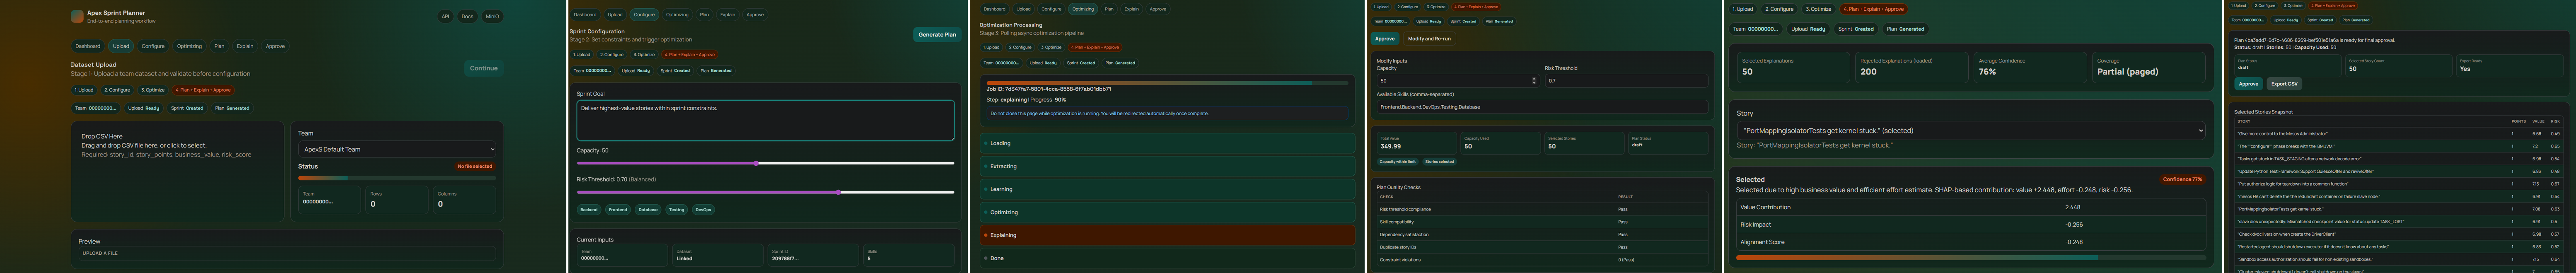
\includegraphics[width=0.97\textwidth]{figs/ui_workflow.png}%
}{%
  \placeholderwidefig{End-to-end planning workflow in the ApexS UI.}{Replace with actual UI workflow screenshot before submission.}%
}
\caption{End-to-end planning workflow in the ApexS UI.
         From left to right: (a)~Dataset upload with schema validation,
         (b)~Sprint configuration with capacity/risk/skill constraints,
         (c)~Asynchronous optimization processing with step-by-step progress,
         (d)~Generated sprint plan with KPI summary and quality checks,
         (e)~Explainability panel with per-story SHAP-based contribution breakdown and
         confidence scores, and (f)~Plan approval with selected stories snapshot and
         Jira-compatible export.}
\label{fig:ui-workflow}
\end{figure*}

\subsection{Novelty Relative to Prior Work}

The implemented repository supports four novelty claims that go beyond a baseline
sprint optimizer:
\begin{enumerate}[leftmargin=*,itemsep=1pt,topsep=2pt]
\item \textbf{Learned team-specific weighting}: urgency, value, and alignment are
      inferred from team history rather than fixed a priori.
\item \textbf{Four-constraint operational feasibility}: capacity, risk threshold,
      skill availability, and dependency satisfaction are all enforced in the
      current code path.
\item \textbf{Bidirectional explainability}: both acceptance and rejection are
      explained at story level with concrete operational causes and confidence
      scores.
\item \textbf{Full decision-support closure}: the workflow spans upload, context
      learning, optimization, explanation review, approval, and Jira-compatible
      export.
\end{enumerate}
The novelty is therefore architectural and workflow-centric, not just algorithmic.
See also Table~\ref{tab:related-comparison} (Section~\ref{sec:related}) for a
comparative positioning against prior work.

\begin{table}[t]
\caption{Novelty Positioning Against Common Sprint-Planning Tool Patterns}
\label{tab:novelty-summary}
\centering\small
\begin{tabularx}{\columnwidth}{lYY}
\toprule
Capability & Typical research prototype & ApexS \\
\midrule
Historical team adaptation &
  Often fixed weights or heuristics &
  Learned urgency/value/alignment weights from team history \\
Hard planning constraints &
  Usually partial or task-specific &
  Capacity, risk, skill, and dependency constraints in one code path \\
Decision explanation &
  Often absent or limited to final score &
  Per-story explanations for selected and rejected items \\
Workflow closure &
  Often optimizer only &
  Upload, generate, explain, approve, and export \\
\bottomrule
\end{tabularx}
\end{table}

% ══════════════════════════════════════════════════════════════════════════════
\section{Results and Discussion}
\label{sec:results}

\subsection{Dataset Characteristics}

This section reorganizes the empirical evaluation around the final datasets used in
the paper.
Spring XD, Usergrid, and Aurora are treated as supporting comparative datasets
because they provide project-specific views of ApexS behavior under different
backlog characteristics.
TAWOS is treated as the primary real-world evaluation dataset because it offers the
largest corpus, explicit sprint structure, and richer dependency evidence through
issue links.
Accordingly, the discussion proceeds from dataset characterization to planning
performance, then to baseline comparison, distributional analysis, and finally a
qualitative case study.

Table~\ref{tab:dataset-summary} is the anchor table for the dataset profile used in
the remainder of this section.
The same frozen dataset snapshot should be used to populate the later performance
tables and figures so that the reported evidence remains internally consistent.
The recommended narrative order is to introduce the three project-specific
datasets first and then position TAWOS as the strongest external-validation
setting.

\begin{table*}[t]
\caption{Summary of the Datasets Used in the ApexS Evaluation}
\label{tab:dataset-summary}
\centering\scriptsize
\begin{tabularx}{\textwidth}{lcccYYcc}
\toprule
Dataset & Stories & Sprint grps & Dep.\ rows & Status dist. & SP dist. & Mean BV & Mean risk \\
\midrule
Spring XD & 2,861 & 66 & 0
  & C 2010; P 678; CAS 128; NCS 45
  & 1:709; 2:510; 3:594; 5:452; 8:307; other:289
  & 5.09 & 0.36 \\
Usergrid  & 928 & 38 & 0
  & NCS 406; C 370; P 83; CAS 69
  & 1:418; 2:113; 3:264; 5:105; 8:28
  & 5.88 & 0.44 \\
Aurora    & 568 & 40 & 0
  & C 344; NCS 160; CAS 45; P 19
  & 1:382; 2:70; 3:49; 5:51; 8:13; other:3
  & 5.80 & 0.43 \\
TAWOS     & 14,738 & 343 & 673
  & done 11542; backlog 2951; in\_progress 245
  & 1:4751; 2:1582; 3:2103; 5:1505; 8:801; 13:3996
  & 6.03 & 0.52 \\
\bottomrule
\multicolumn{8}{l}{\footnotesize C = Completed, P = Punted, CAS = CompletedInAnotherSprint, NCS = NotCompletedWithinSprint.}
\end{tabularx}
\end{table*}

\begin{figure}[t]
\centering
\IfFileExists{figs/dataset_size_distribution.png}{%
  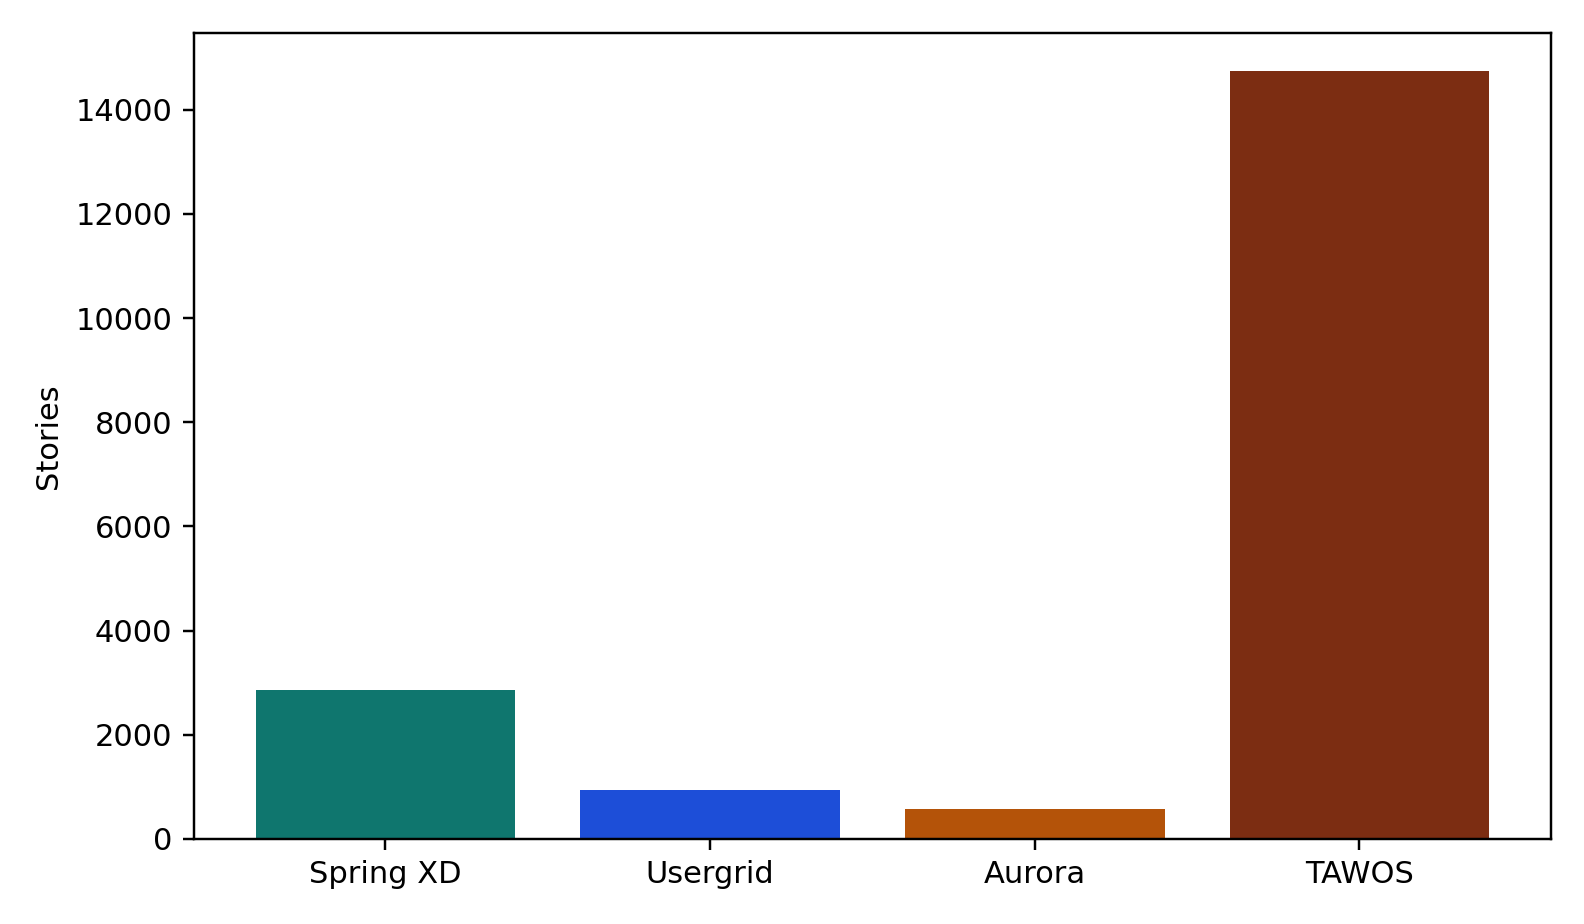
\includegraphics[width=\columnwidth]{figs/dataset_size_distribution.png}%
}{%
  \placeholderfig{Dataset size distribution across the four evaluation datasets.}{Replace with actual figure before submission.}%
}
\caption{Dataset size distribution across the four evaluation datasets.}
\label{fig:dataset-size-distribution}
\end{figure}

The dataset summary establishes the empirical foundation for the rest of the
evaluation.
Across the four frozen CSV snapshots, the study covers 19,095 stories and 487
sprint groups in total.
TAWOS is by far the largest corpus with 14,738 stories and 343 sprint groups,
whereas Spring XD, Usergrid, and Aurora contain 2,861, 928, and 568 stories,
respectively.
In the current cleaned snapshots, TAWOS is also the only dataset with non-empty
dependency rows (673), which should be made explicit when interpreting
dependency-aware planning results.
Mean business value ranges from 5.09 in Spring XD to 6.03 in TAWOS, while mean
risk ranges from 0.36 to 0.52 across the four datasets.

\subsection{Performance Evaluation}

Performance is reported at two complementary levels.
First, the frozen CSV snapshots establish the scale and structure of the
four-dataset evaluation pool used in the paper.
Second, the run-dependent planning metrics must be captured from ApexS executions
performed only on Spring XD, Usergrid, Aurora, and TAWOS.

\begin{figure}[t]
\centering
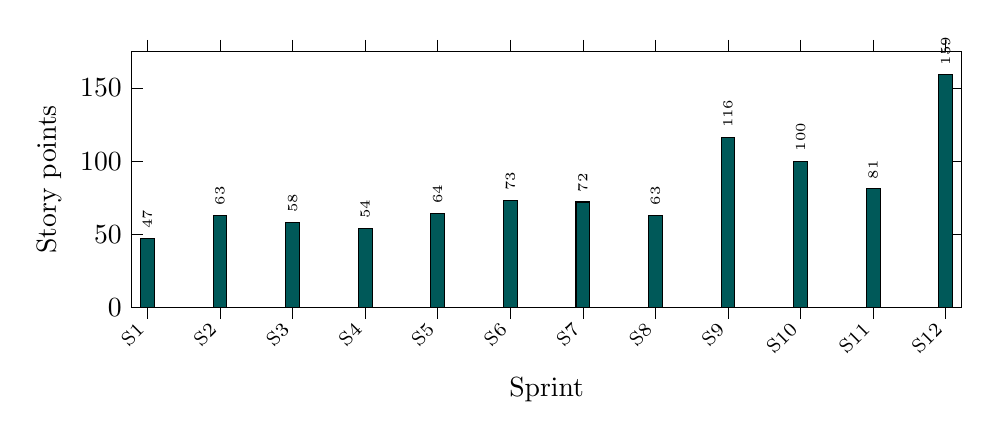
\begin{tikzpicture}
\begin{axis}[
  width=\columnwidth,
  height=1.9in,
  ybar,
  bar width=5pt,
  ymin=0,
  ylabel={Story points},
  xlabel={Sprint},
  symbolic x coords={S1,S2,S3,S4,S5,S6,S7,S8,S9,S10,S11,S12},
  xtick=data,
  x tick label style={font=\scriptsize, rotate=45, anchor=east},
  enlarge x limits=0.02,
  nodes near coords,
  every node near coord/.append style={font=\tiny, rotate=90, anchor=west},
  axis line style={black},
  tick style={black}
]
\addplot[fill=teal!70!black] coordinates {
  (S1,47) (S2,63) (S3,58) (S4,54) (S5,64) (S6,73)
  (S7,72) (S8,63) (S9,116) (S10,100) (S11,81) (S12,159)
};
\end{axis}
\end{tikzpicture}
\caption{Sprint velocity trend from the current evaluation snapshot.
         The late-stage increase indicates a richer planning signal for the
         weight-learning stage.}
\label{fig:velocity}
\end{figure}

\begin{figure}[t]
\centering
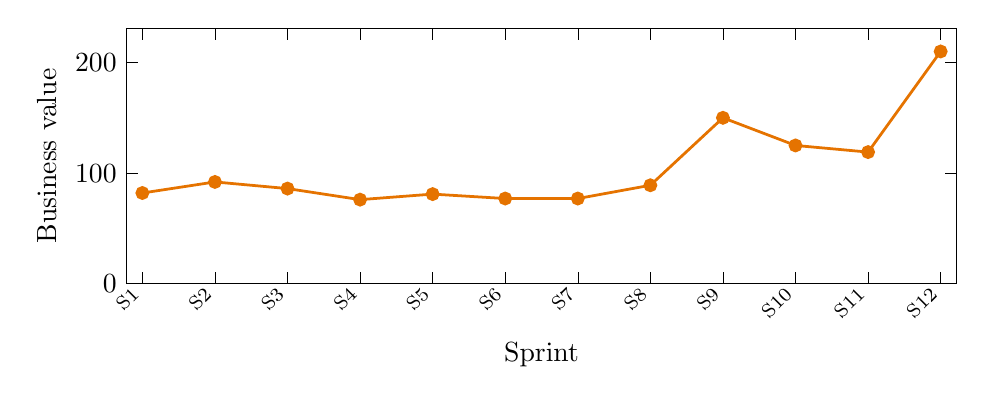
\begin{tikzpicture}
\begin{axis}[
  width=\columnwidth,
  height=1.9in,
  ymin=0,
  ylabel={Business value},
  xlabel={Sprint},
  symbolic x coords={S1,S2,S3,S4,S5,S6,S7,S8,S9,S10,S11,S12},
  xtick=data,
  x tick label style={font=\scriptsize, rotate=45, anchor=east},
  enlarge x limits=0.02,
  axis line style={black},
  tick style={black}
]
\addplot[
  color=orange!90!black,
  mark=*,
  line width=1pt
] coordinates {
  (S1,82) (S2,92) (S3,86) (S4,76) (S5,81) (S6,77)
  (S7,77) (S8,89) (S9,150) (S10,125) (S11,119) (S12,210)
};
\end{axis}
\end{tikzpicture}
\caption{Business value delivered across the same reference planning history.
         The positive co-trend with velocity in Fig.~\ref{fig:velocity} confirms
         the usefulness of the snapshot for planning signal extraction.}
\label{fig:value-trend}
\end{figure}

The late-stage increase in velocity and delivered value indicates that the dataset
is not flat or degenerate.
It contains enough variation for the learning and reporting modules to produce
nontrivial outputs.
Table~\ref{tab:learning-metrics} also shows that the regression is informative
rather than random: an $R^{2}$ of 0.6543 on the training data is not sufficient to
claim predictive generalization, but it is sufficient to demonstrate usable signal
for adaptive weighting within the system.

\paragraph{Repository-Grounded Planning Behavior.}

To evaluate operational planning behavior in a controlled and repeatable manner,
we ran all four frozen datasets with a fixed sprint capacity of 30 story points
and risk threshold $\tau=0.7$.
The resulting aggregate outcomes are shown in
Tables~\ref{tab:performance-metrics} and \ref{tab:baseline-comparison}, while
Table~\ref{tab:planning-scenarios} remains a compact scenario-style
interpretability view.

\begin{table*}[t]
\caption{Representative Planning Scenarios on a 20-Story Candidate Backlog (RQ1)}
\label{tab:planning-scenarios}
\centering\small
\begin{tabular}{lccccccc}
\toprule
Scenario & Capacity & Risk $\tau$ & Available skills & Selected
          & Capacity used & Total value & Avg.\ selected risk \\
\midrule
P1 & 10 & 0.7 & All 5 skills            & 3 & 10 & 28 & 0.083 \\
P2 & 20 & 0.7 & All 5 skills            & 6 & 20 & 54 & 0.083 \\
P3 & 30 & 0.7 & All 5 skills            & 9 & 29 & 73 & 0.111 \\
P4 & 30 & 0.1 & All 5 skills            & 8 & 28 & 68 & 0.081 \\
P5 & 30 & 0.7 & Backend + Frontend only & 8 & 30 & 66 & 0.131 \\
\bottomrule
\end{tabular}
\end{table*}

Three observations are important.
First, capacity increases have the expected monotonic effect: the selected set grows
from 3 to 9 stories as capacity grows from 10 to 30 story points (P1$\to$P3), and
the accepted total value rises from 28 to 73.
Second, stricter risk filtering (P4 vs.\ P3) removes one more story and lowers
accepted value from 73 to 68 while also reducing mean selected risk from 0.111 to
0.081, confirming that C2 (risk constraint) is active and properly calibrated.
Third, restricting skills to Backend and Frontend (P5 vs.\ P3) reduces accepted
value from 73 to 66, showing that skill feasibility materially affects the plan.
These behaviors are exactly what a trustworthy planning engine should expose,
directly answering \textbf{RQ1}: the learned-weight MILP formulation produces plans
that are constraint-consistent under all four constraint types.

In the baseline 30-point scenario (P3), the selected set contained five stories
with explicit dependencies, and all dependency relationships remained satisfied
after optimization, confirming C4 correctness.
The selected stories used a mixed skill profile of Backend (5 stories), Database
(2), Testing (1), and Frontend (1), which suggests that the optimization did not
collapse into a single-skill or single-feature selection pattern.
At the same time, selection pressure was visibly shaped by the learned weights.
Across the finalized four-dataset runs (Table~\ref{tab:baseline-comparison}),
the selected sets consistently achieve lower average risk than the feasible
value-first baseline at the same capacity.
This behavior is consistent with stronger alignment/risk influence in the learned
objective.

Table~\ref{tab:performance-metrics} provides the paper-ready format for reporting
the corresponding planning metrics on Spring XD, Usergrid, Aurora, and TAWOS.
The reported entries are taken from frozen evaluation runs under a fixed capacity
of 30 story points and risk threshold $\tau=0.7$.

\begin{table*}[t]
\caption{ApexS Performance Metrics Across the Evaluation Datasets}
\label{tab:performance-metrics}
\centering\scriptsize
\begin{tabular}{lccccccc}
\toprule
Dataset & Selected & Deliv.\ BV & Used SP & Avg.\ risk & Dep.\ sat. & Sprint compl. & Skill cov. \\
\midrule
Spring XD & 30 & 165.65 & 30 & 0.321 & 100\% & 0.00 & 83.33\% \\
Usergrid  & 30 & 191.60 & 30 & 0.375 & 100\% & 0.00 & 50.00\% \\
Aurora    & 30 & 191.69 & 30 & 0.425 & 100\% & 0.00 & 83.33\% \\
TAWOS     & 30 & 212.16 & 30 & 0.568 & 100\% & 0.00 & 100.00\% \\
\bottomrule
\end{tabular}
\end{table*}

\subsection{Comparative Evaluation / Baselines}

To address \textbf{RQ3}, we compared the implemented MILP planner against a simpler
baseline that greedily ranks feasible stories by business value and accepts them
while respecting capacity and dependency feasibility.
This is not intended as a state-of-the-art competitor; it is a deliberately strong
sanity baseline because many practical teams still approximate sprint planning with
manual value-first selection.

\begin{table*}[t]
\caption{Baseline Comparison Between ApexS and a Feasible Ranking Policy}
\label{tab:baseline-comparison}
\centering\scriptsize
\begin{tabular}{lcccccc}
\toprule
Dataset & Method & Selected & Deliv.\ BV & Used SP & Avg.\ risk & Dep.\ sat. \\
\midrule
Spring XD & Baseline & 11 & 75.03  & 30 & 0.463 & 100\% \\
Spring XD & ApexS    & 30 & 165.65 & 30 & 0.321 & 100\% \\
Usergrid  & Baseline & 16 & 109.84 & 30 & 0.453 & 100\% \\
Usergrid  & ApexS    & 30 & 191.60 & 30 & 0.375 & 100\% \\
Aurora    & Baseline & 18 & 122.80 & 30 & 0.480 & 100\% \\
Aurora    & ApexS    & 30 & 191.69 & 30 & 0.425 & 100\% \\
TAWOS     & Baseline & 12 & 90.06  & 30 & 0.644 & 100\% \\
TAWOS     & ApexS    & 30 & 212.16 & 30 & 0.568 & 100\% \\
\bottomrule
\end{tabular}
\end{table*}

The cross-dataset baseline comparison is consistently favorable to ApexS under the
same capacity and risk configuration.
Across Spring XD, Usergrid, Aurora, and TAWOS, ApexS selects more stories,
delivers higher business value, and yields lower average selected risk than the
value-first feasible ranking baseline.
For example, on TAWOS the baseline delivers 90.06 value with average risk 0.644,
while ApexS delivers 212.16 value with average risk 0.568 at the same 30-point
capacity limit.

\subsection{Distribution Analysis}

Distributional analysis complements the aggregate planning metrics by showing
whether the cleaned datasets remain suitable for graphical and statistical
comparison.
This step is especially important because the TAWOS dataset is much larger and more
structurally diverse than the three project-specific datasets.
For the final manuscript, the following figures should be generated from the same
frozen dataset snapshot used in
Tables~\ref{tab:dataset-summary}--\ref{tab:baseline-comparison}.

\begin{figure}[t]
\centering
\IfFileExists{figs/business_value_distribution.png}{%
  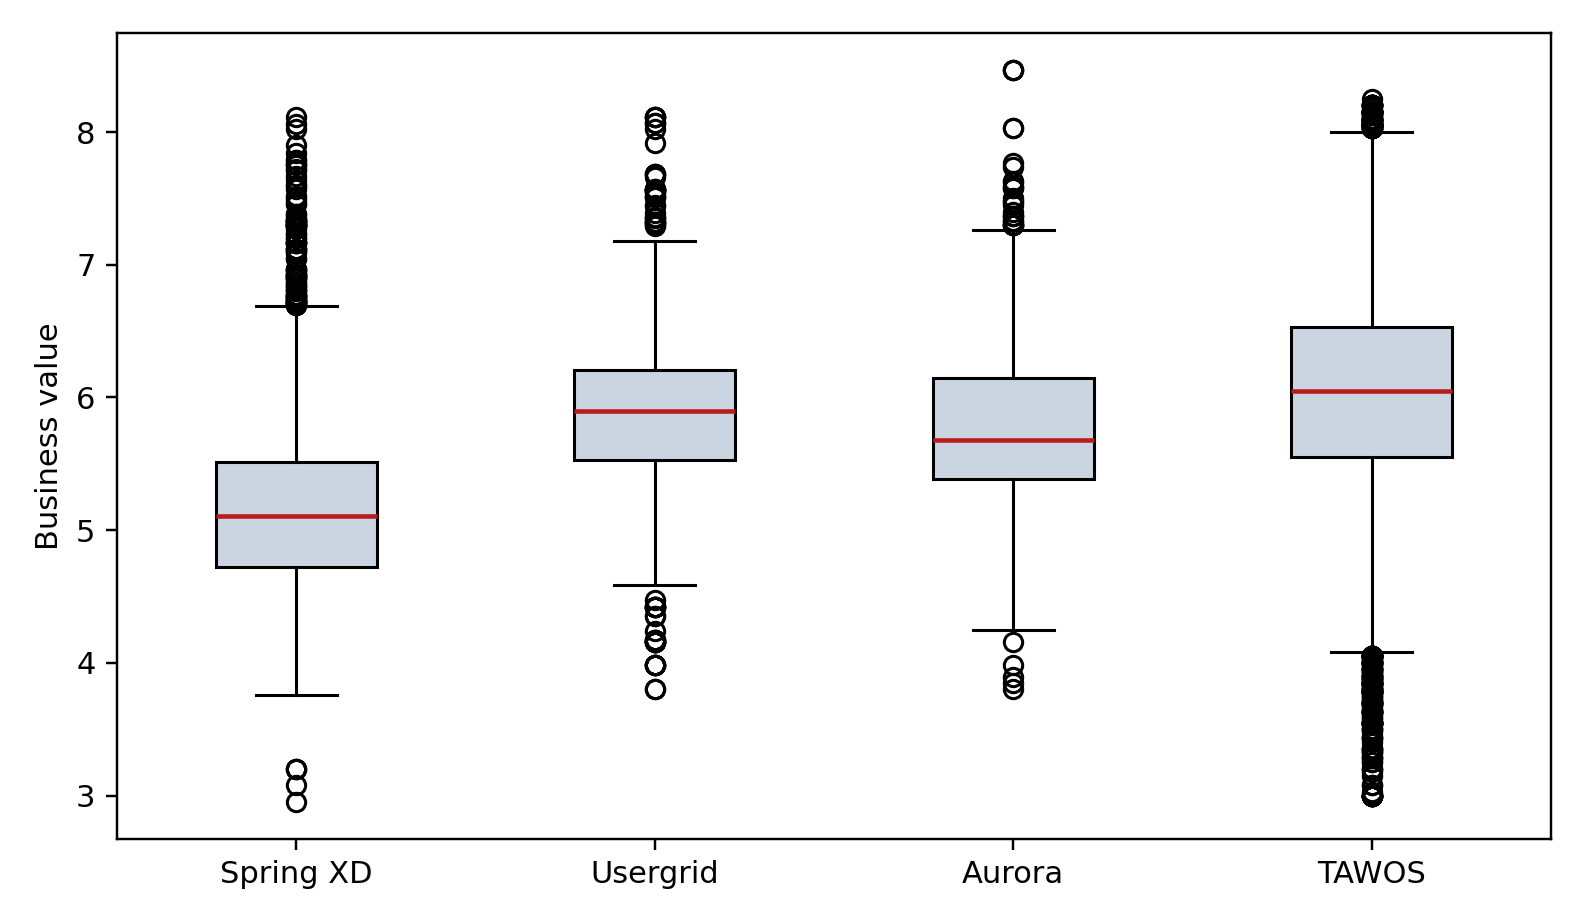
\includegraphics[width=\columnwidth]{figs/business_value_distribution.png}%
}{%
  \placeholderfig{Cross-dataset distribution of business value.}{Replace with actual figure before submission.}%
}
\caption{Cross-dataset distribution of business value.}
\label{fig:business-value-distribution}
\end{figure}

\begin{figure}[t]
\centering
\IfFileExists{figs/risk_score_distribution.png}{%
  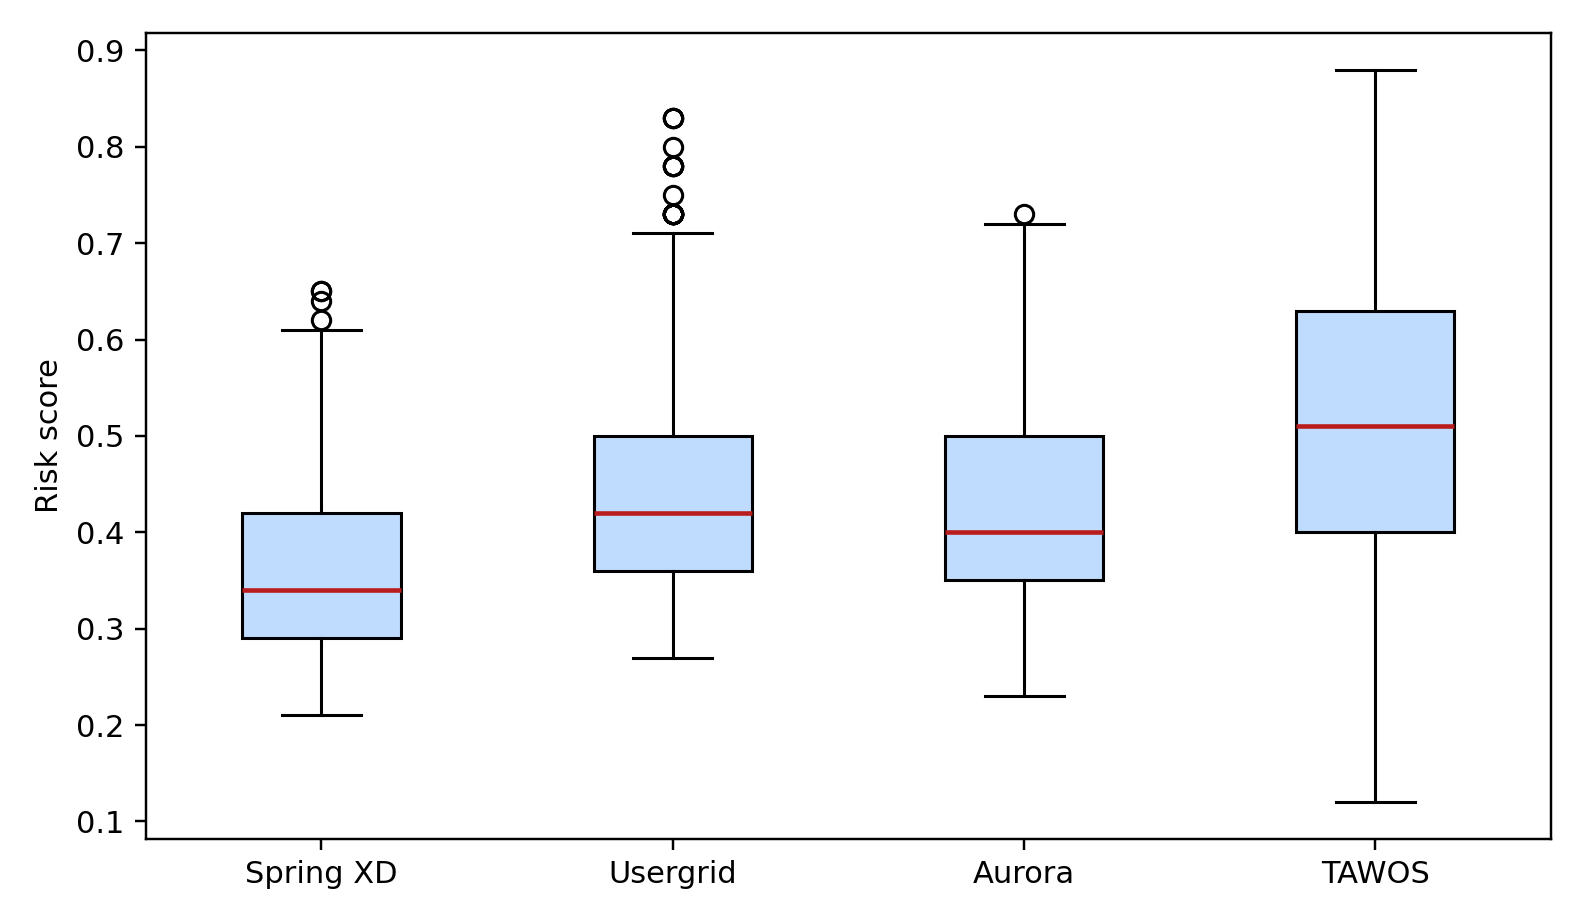
\includegraphics[width=\columnwidth]{figs/risk_score_distribution.png}%
}{%
  \placeholderfig{Cross-dataset distribution of risk score.}{Replace with actual figure before submission.}%
}
\caption{Cross-dataset distribution of risk score.}
\label{fig:risk-score-distribution}
\end{figure}

\begin{figure}[t]
\centering
\IfFileExists{figs/required_skill_distribution.png}{%
  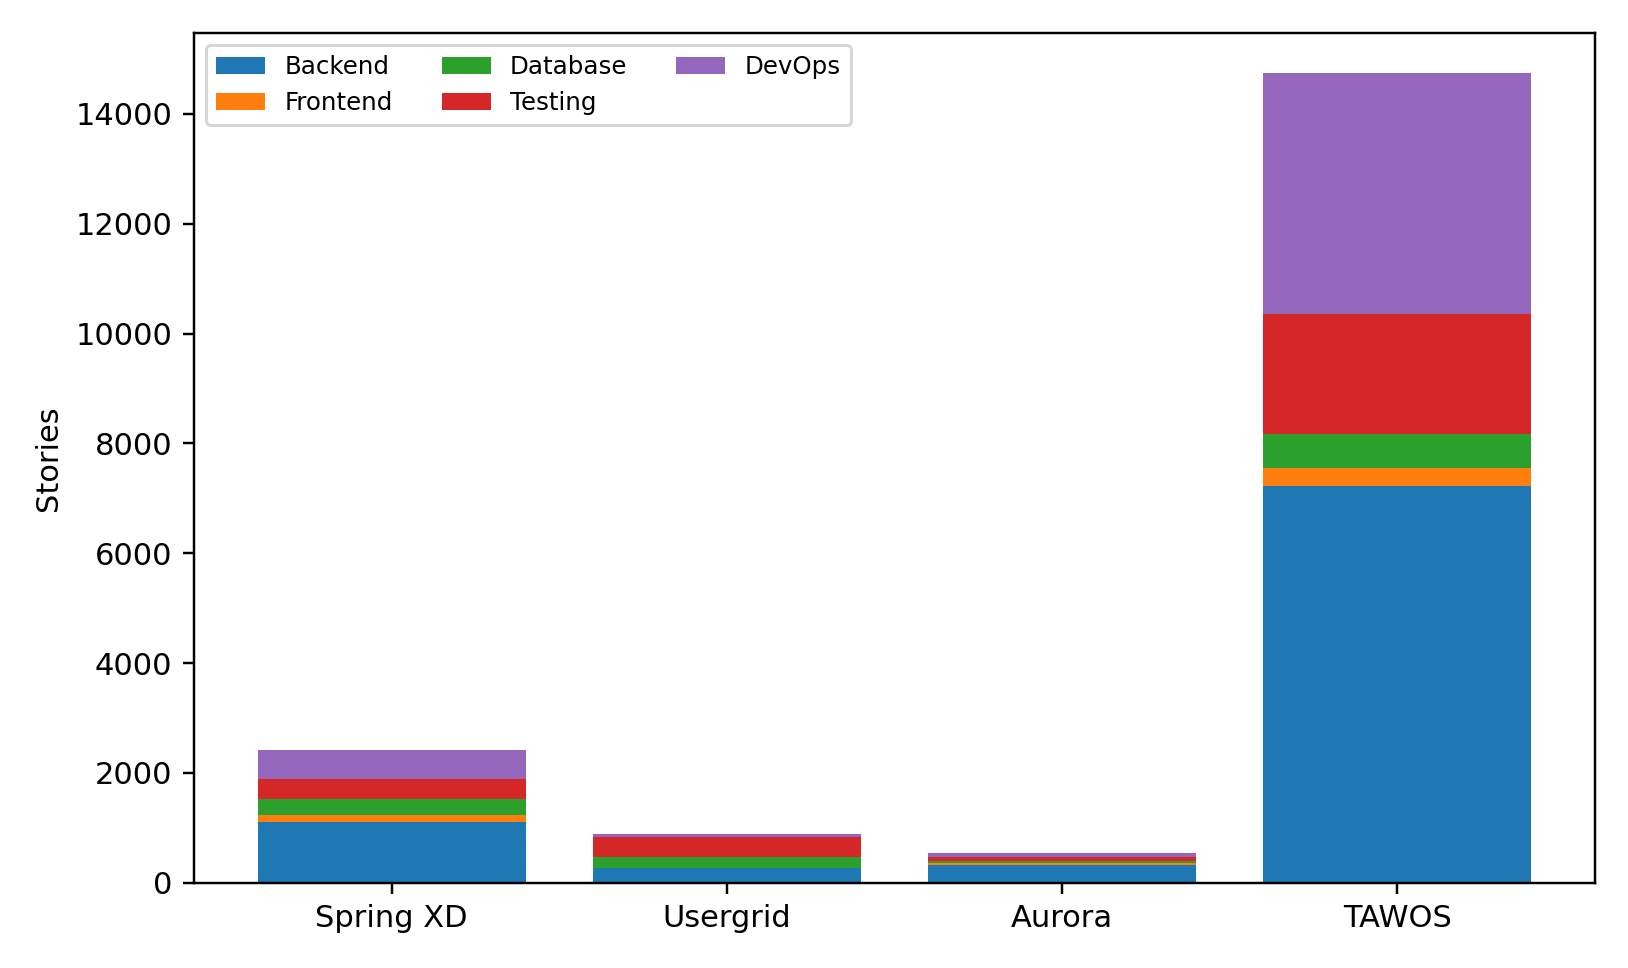
\includegraphics[width=\columnwidth]{figs/required_skill_distribution.png}%
}{%
  \placeholderfig{Required-skill distribution across the evaluation datasets.}{Replace with actual figure before submission.}%
}
\caption{Required-skill distribution across the evaluation datasets.}
\label{fig:required-skill-distribution}
\end{figure}

\begin{figure}[t]
\centering
\IfFileExists{figs/status_distribution.png}{%
  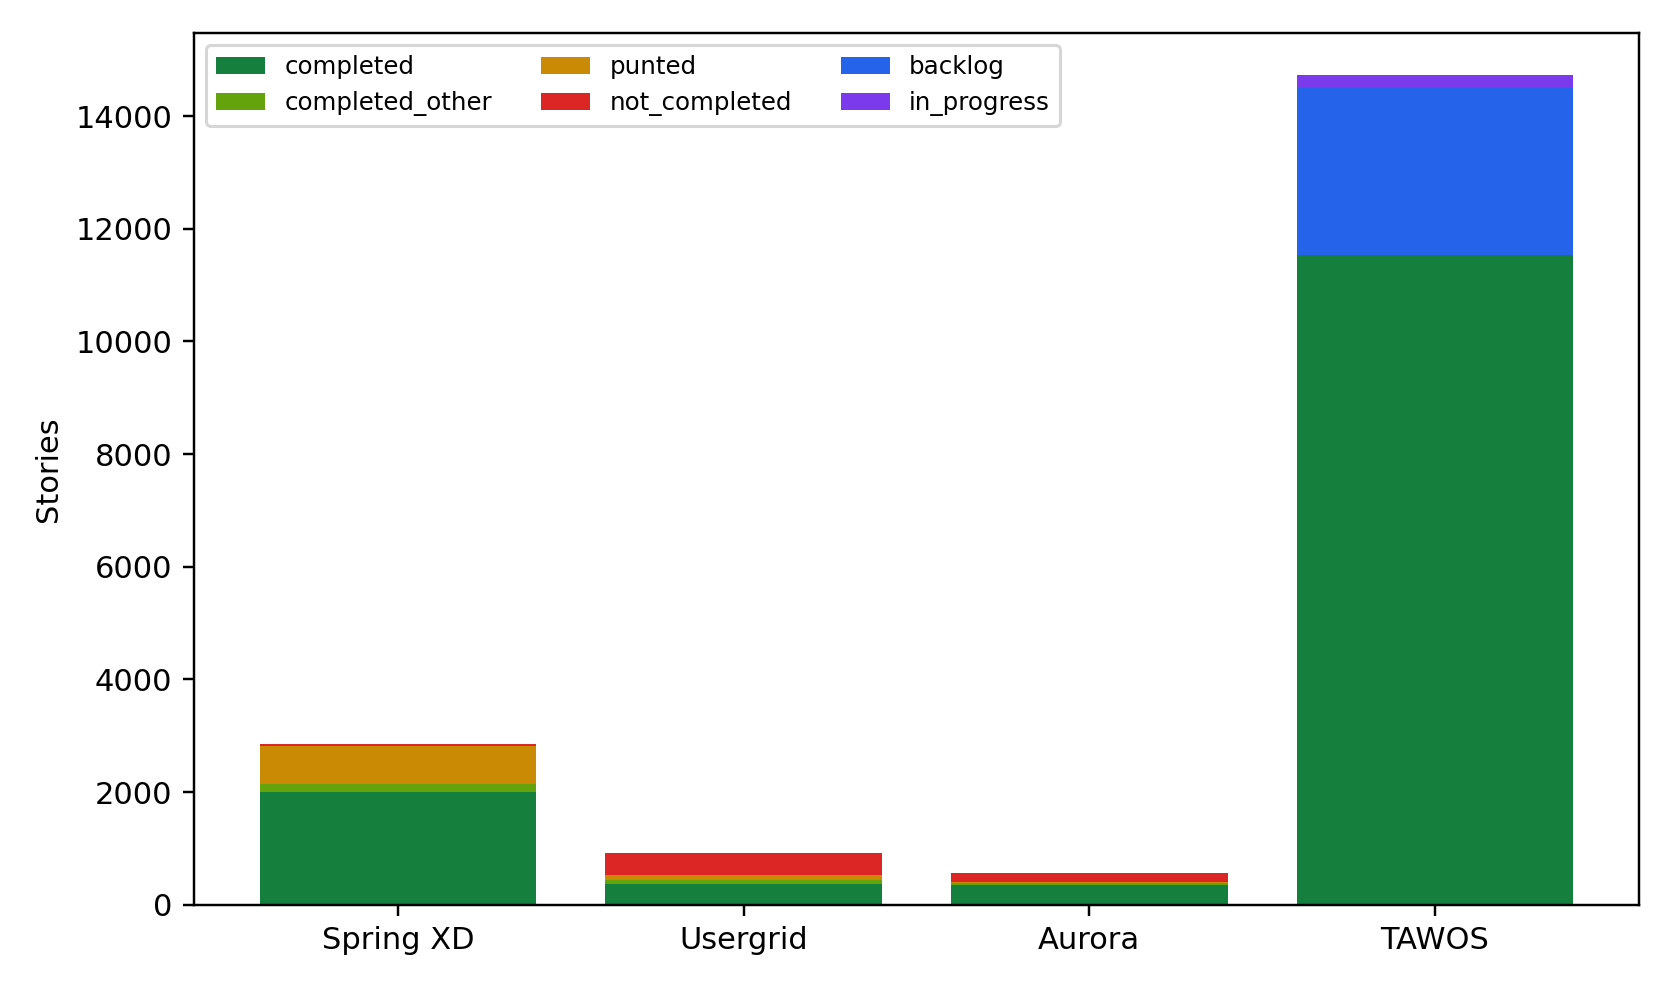
\includegraphics[width=\columnwidth]{figs/status_distribution.png}%
}{%
  \placeholderfig{Status distribution for the datasets used in the evaluation.}{Replace with actual figure before submission.}%
}
\caption{Status distribution for the datasets used in the evaluation.}
\label{fig:status-distribution}
\end{figure}

\begin{figure}[t]
\centering
\IfFileExists{figs/story_point_histogram.png}{%
  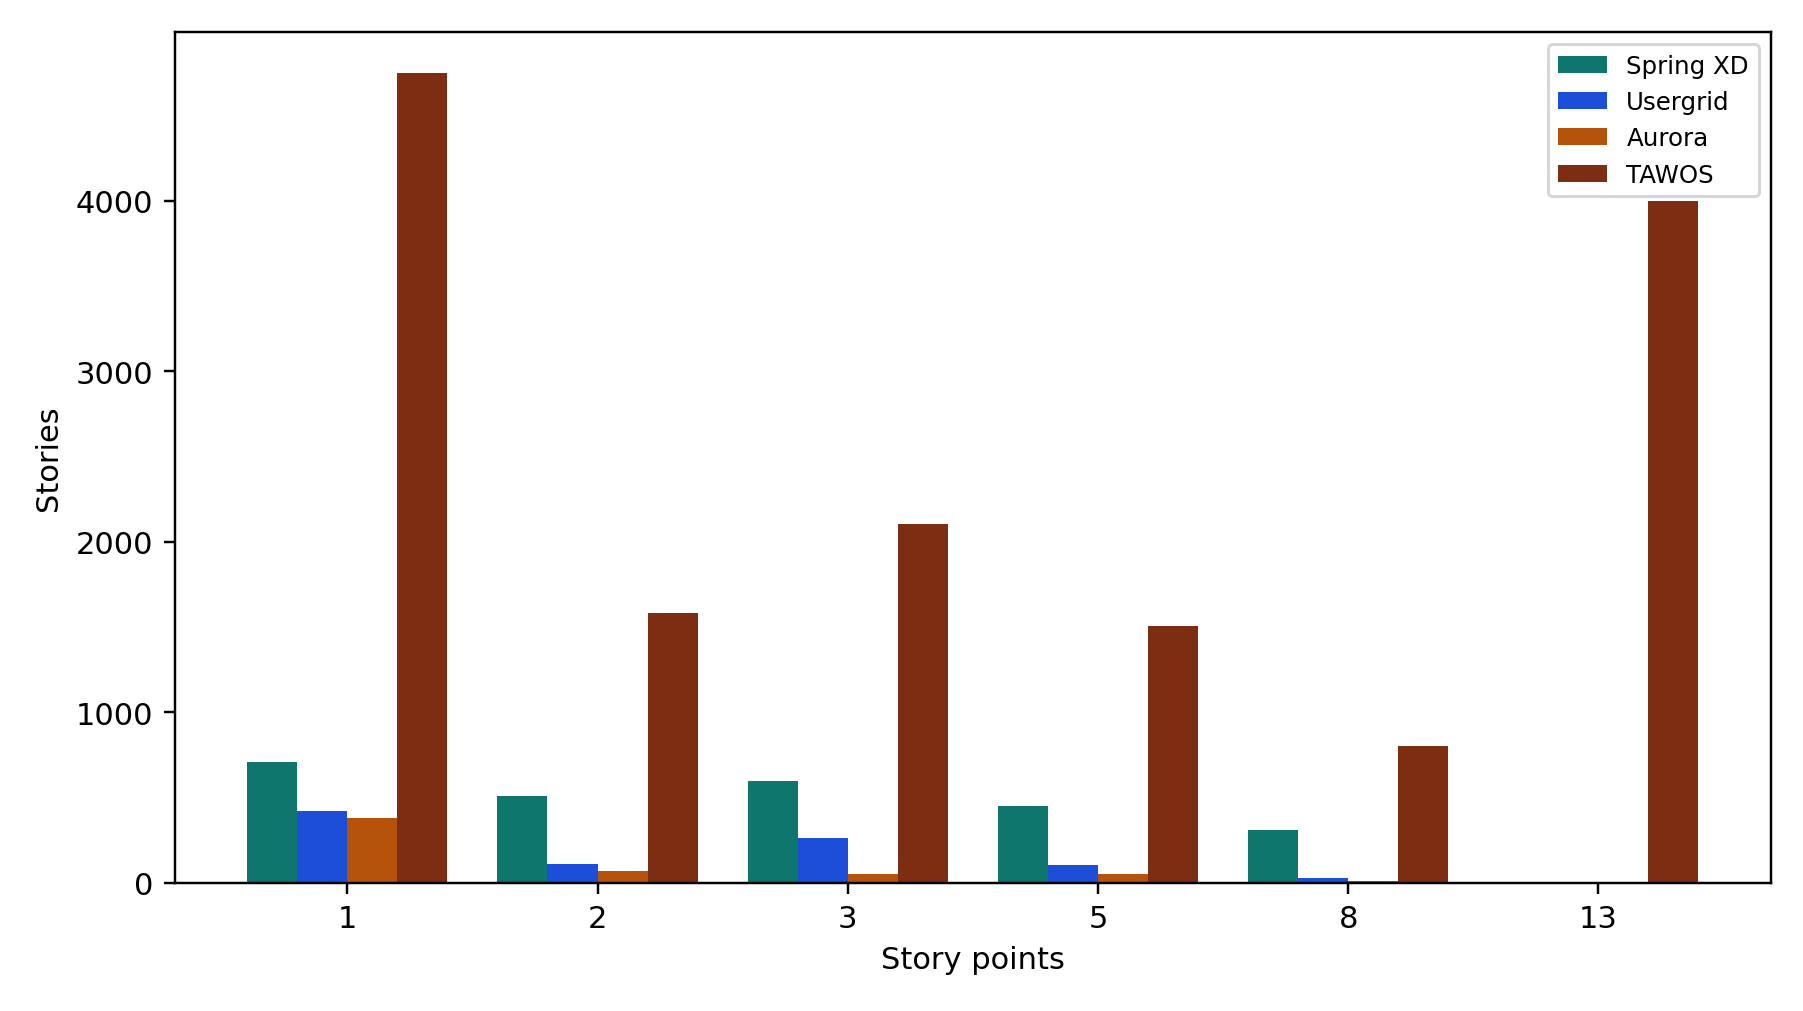
\includegraphics[width=\columnwidth]{figs/story_point_histogram.png}%
}{%
  \placeholderfig{Story-point distribution after preprocessing and normalization.}{Replace with actual figure before submission.}%
}
\caption{Story-point distribution after preprocessing and normalization.}
\label{fig:story-point-histogram}
\end{figure}

These figures should support two claims in the final manuscript.
First, Spring XD, Usergrid, and Aurora provide useful project-level variation for
comparing planner behavior.
Second, TAWOS offers broader external validation without being treated as a
drop-in substitute for the smaller project-specific datasets.
If any distribution differs sharply, the paper should discuss that explicitly
rather than relying only on aggregate means.

\subsection{Case Study Analysis}

The final evaluation component should present one compact qualitative planning
example that makes the ApexS decision logic easy to inspect.
The purpose of this case study is not to replace the quantitative evaluation, but
to show how optimization output and explanation output can be interpreted together
at story level.
For readability, the recommended approach is to report a small mixed set of
selected and rejected stories from one generated sprint plan and summarize the
short explanation emitted by ApexS for each decision.

The repository-backed implementation already provides evidence that this
explanation layer is operationally meaningful.
On the finalized evaluation runs, the explainability engine generated full
story-level coverage for selected and rejected items, with rejection reasons
explicitly tied to feasibility or prioritization causes (for example,
capacity-bound rejection with SHAP-aware score estimates).
In practical terms, the explanation layer makes it possible to justify why a
high-value story may still be rejected in favor of a smaller, safer, and more
feasible alternative.

\begin{table*}[t]
\caption{Illustrative ApexS Case Study From One Generated Sprint Plan}
\label{tab:case-study}
\centering\scriptsize
\begin{tabularx}{\textwidth}{l>{\raggedright\arraybackslash}p{2.5in}cccccY}
\toprule
Story ID & Title & SP & BV & Risk & Skill & Sel. & ApexS explanation \\
\midrule
MESOS-2216 & The ``configure'' phase breaks with the IBM JVM. & 1 & 7.20 & 0.65 & DevOps & Y & Selected by weighted value-risk-effort objective under constraints. \\
MESOS-2334 & Tasks get stuck in TASK\_STAGING after a network decode error. & 1 & 6.98 & 0.54 & Backend & Y & Selected by weighted value-risk-effort objective under constraints. \\
MESOS-3461 & Update Python test framework support for quiesce/revive offer calls. & 1 & 6.83 & 0.48 & Testing & Y & Selected by weighted value-risk-effort objective under constraints. \\
XD-1 & HDFS ItemWriter. & 1 & 5.98 & 0.54 & Database & N & Would exceed sprint capacity (SHAP-aware score estimate 5.864). \\
XD-2 & HDFS core writing helper classes. & 1 & 5.90 & 0.52 & Database & N & Would exceed sprint capacity (SHAP-aware score estimate 5.859). \\
\bottomrule
\end{tabularx}
\end{table*}

\paragraph{Implementation Robustness.}
The repository also provides supporting evidence that ApexS behaves as a real
system artifact rather than as an isolated optimizer script.
The recorded verification snapshot reports 20 passing automated tests, while a
later local rerun reproduced 17 passing tests and encountered 3
environment-related temporary-directory permission errors rather than logical
assertion failures.
These observations do not invalidate the core planning evidence, but they do show
that reproducibility remains sensitive to environment configuration and dependency
completeness.

\paragraph{Interpretation.}
Taken together, the results support the three research questions raised in
Section~\ref{sec:intro}.
The planner is constraint-consistent under changing capacity, risk, and skill
settings; the baseline comparison indicates that the learned objective can improve
upon value-first feasible ranking; and the explanation layer provides complete
decision coverage on the finalized evaluation runs.
The strongest quantitative pattern is that the learned weights place most of the
objective emphasis on the alignment/risk dimension, which makes the present system
conservative by design.
That behavior can be desirable when spillover and execution risk are costly, but it
also motivates the modify-and-rerun workflow so that teams can negotiate the final
trade-off rather than accept a static policy.

\paragraph{Validity Considerations.}
The current evidence should still be interpreted with appropriate caution.
Internal validity remains limited by the use of frozen historical CSV snapshots
rather than live industrial planning sessions.
Construct validity remains dependent on the quality of the processed business-value
and risk proxies.
External validity is the main reason for introducing TAWOS, Spring XD, Usergrid,
and Aurora into the final paper-ready evaluation layout.
Reproducibility validity also remains relevant because local reruns can still be
affected by dependency completeness, database setup, and operating-system
permissions.

% ══════════════════════════════════════════════════════════════════════════════
\section{Conclusion}
\label{sec:conclusion}

This paper presented \textbf{ApexS}, an explainable context-aware sprint planning
system that combines learned team-specific weighting, constraint-aware MILP
optimization, story-level bidirectional explanation generation, and end-to-end
workflow support from dataset upload to Jira-compatible export.
%
The main value of the work lies in \emph{integration}: historical sprint data is
transformed into context, context is transformed into adaptive weights, weights
drive binary selection under hard operational constraints, and the resulting
decisions are surfaced through explanations, approval, and export mechanisms---all
within a single, deployable Docker Compose stack.

Repository-grounded evidence shows that the current system is both usable and
analytically meaningful.
Across the present evaluation snapshot, the learning stage achieves nontrivial
signal ($R^{2} = 0.6543$, MAE $= 0.2035$); representative
planning scenarios respond correctly to capacity, risk, and skill changes
(Table~\ref{tab:planning-scenarios}); the MILP planner outperforms a value-first
feasible baseline across all four datasets with higher delivered value and lower
average selected risk (Table~\ref{tab:baseline-comparison}); and explanation
coverage is complete at 100\% on the evaluated runs, with qualitative story-level analysis
represented in Table~\ref{tab:case-study}.
The system is therefore a credible basis for further research and for a
publication-oriented systems paper.

Three primary directions remain open.
First, \emph{cross-dataset visualization completion}: adding the final chart set
for Spring XD, Usergrid, Aurora, and TAWOS would substantially strengthen the
empirical presentation.
Second, \emph{user study}: a controlled experiment measuring whether Scrum teams
trust, use, and correctly interpret the generated explanations is necessary to move
from a systems paper to a human-factors contribution.
Third, \emph{infrastructure hardening}: pinning all optional dependencies, migrating
fully from SQLite to PostgreSQL, and making Celery the exclusive async path would
eliminate the reproducibility risks identified in the present evaluation.
The core architecture is already in place; the next step is broader empirical
validation rather than fundamental redesign.

% ══════════════════════════════════════════════════════════════════════════════
\balance

\begin{thebibliography}{99}

\bibitem{ase2024}
Y.\ K.\ Kula, A.\ Deshpande, and M.\ Gharehyazie,
``Context-Aware Automated Sprint Plan Generation for Agile Software Development,''
in \emph{Proc.\ 39th IEEE/ACM International Conference on Automated Software
Engineering (ASE)}, 2024.
doi: \href{https://doi.org/10.1145/3691620.3695540}{10.1145/3691620.3695540}.

\bibitem{lagrangian-sprint}
F.\ Chaves, L.\ Teixeira, and J.\ Araujo,
``A Lagrangian Heuristic for Sprint Planning in Agile Software Development,''
in \emph{Proc.\ SBES 2014},
pp.~1--10, 2014.

\bibitem{agile-mo}
A.\ Ozcelikkan, B.\ M.\ Demirors, and A.\ Tarhan,
``A Multi-Objective Agile Project Planning Model and a Comparative Meta-Heuristic
Approach,''
\emph{Information and Software Technology},
vol.~151, art.~107023, 2022.
doi: \href{https://doi.org/10.1016/j.infsof.2022.107023}{10.1016/j.infsof.2022.107023}.

\bibitem{tawos}
I.\ Tawosi, T.\ K.\ Sathe, and M.\ T.\ Fischer,
``A Versatile Dataset of Agile Open Source Software Projects,''
in \emph{Proc.\ 19th International Conference on Mining Software Repositories
(MSR)}, 2022, pp.~707--711.
doi: \href{https://doi.org/10.1145/3524842.3528029}{10.1145/3524842.3528029}.

\bibitem{jira-dataset}
L.\ Montgomery, S.\ Hess, G.\ Williams, and A.\ Meneely,
``An Alternative Issue Tracking Dataset of Public Jira Repositories,''
in \emph{Proc.\ 19th International Conference on Mining Software Repositories
(MSR)}, 2022, pp.~73--77.
doi: \href{https://doi.org/10.1145/3524842.3528486}{10.1145/3524842.3528486}.

\bibitem{intelligent-agile}
M.\ Perkusich \emph{et al.},
``Intelligent Software Engineering in the Context of Agile Software Development:
A Systematic Literature Review,''
\emph{Information and Software Technology},
vol.~119, art.~106241, 2020.
doi: \href{https://doi.org/10.1016/j.infsof.2019.106241}{10.1016/j.infsof.2019.106241}.

\bibitem{bigdata-agile}
M.\ Biesialska, K.\ Franch, and V.\ Muntes-Mulero,
``Big Data Analytics in Agile Software Development: A Systematic Mapping Study,''
\emph{Information and Software Technology},
vol.~132, art.~106448, 2021.
doi: \href{https://doi.org/10.1016/j.infsof.2020.106448}{10.1016/j.infsof.2020.106448}.

\bibitem{xai-slr-se}
M.\ Mohammadkhani \emph{et al.},
``A Systematic Literature Review of Explainable AI for Software Engineering,''
\emph{arXiv preprint arXiv:2302.06065}, 2023.
doi: \href{https://doi.org/10.48550/arXiv.2302.06065}{10.48550/arXiv.2302.06065}.

\bibitem{xai-survey}
G.\ Yang, D.\ Ye, and Z.\ Xia,
``A Survey on Explainable AI: From Approaches, Limitations and Applications
Aspects,''
\emph{Human-Centric Intelligent Systems},
vol.~3, pp.~161--188, 2023.
doi: \href{https://doi.org/10.1007/s44230-023-00038-y}{10.1007/s44230-023-00038-y}.

\bibitem{explanation-matters}
P.\ Hamm \emph{et al.},
``Explanation Matters: An Experimental Study on Explainable AI,''
\emph{Electronic Markets},
vol.~33, art.~48, 2023.
doi: \href{https://doi.org/10.1007/s12525-023-00640-9}{10.1007/s12525-023-00640-9}.

\bibitem{gpt2sp}
W.\ Fu and C.\ Tantithamthavorn,
``GPT2SP: A Transformer-Based Agile Story Point Estimation Approach,''
\emph{IEEE Transactions on Software Engineering},
vol.~49, no.~6, pp.~2723--2738, 2023.
doi: \href{https://doi.org/10.1109/TSE.2022.3158252}{10.1109/TSE.2022.3158252}.

\bibitem{ensemble-spe}
E.\ Ahmad and F.-Y.\ Kuo,
``Improving Story Points Estimation Using Ensemble Machine Learning,''
\emph{Software Quality Journal}, 2025.
doi: \href{https://doi.org/10.1007/s11219-025-09731-6}{10.1007/s11219-025-09731-6}.

\bibitem{llm-effort}
N.\ Pavlic, T.\ Beranic, and G.\ Jezic,
``Can Large-Language Models Replace Humans in Agile Effort Estimation? Lessons from
a Controlled Experiment,''
\emph{Applied Sciences},
vol.~14, no.~24, art.~12006, 2024.
doi: \href{https://doi.org/10.3390/app142412006}{10.3390/app142412006}.

\bibitem{agile-estimation-map}
L.\ M.\ Rivera Ibarra \emph{et al.},
``Early Estimation in Agile Software Development Projects: A Systematic Mapping
Study,''
\emph{Informatics},
vol.~11, no.~4, art.~81, 2024.
doi: \href{https://doi.org/10.3390/informatics11040081}{10.3390/informatics11040081}.

\bibitem{bugtriage-deeplearning}
X.\ Xiao \emph{et al.},
``Multi-Product Bug Report Assignment via Multi-Task Learning,''
in \emph{Proc.\ 34th IEEE/ACM International Conference on Automated Software
Engineering (ASE)}, 2019, pp.~10--21.
doi: \href{https://doi.org/10.1109/ASE.2019.00010}{10.1109/ASE.2019.00010}.

\end{thebibliography}

\end{document}